% Provenance (never printed): see sources/outline_sources.md (Year 2: index minerals and zones,
% geothermometers and geobarometers, prograde and retrograde paths, metamorphic series,
% ultrahigh-pressure rocks and exhumation, ocean-floor metamorphism). Garnet-biotite
% calibration refitted from the Ferry and Spear (1978) brackets tabulated by Holdaway et al.
% (1997); GASP from Koziol and Newton (1988); thickening model after England and Thompson
% (1984) in figdata/bachelor-2/ptpaths.py; exercise and problem values in the Book 4 scratch
% calculators calc/ch11.py and calc/ch11b.py.
\chapter{Thermobarometrie en P--T--t-paden}\label{ch:b2:pt-paths}

Een granaat van enkele millimeters, gegroeid in een schist, bewaart in zijn kern de samenstelling
die hij had toen hij begon te groeien en in zijn rand de samenstelling die hij had toen hij ophield. Elke
zone was op dat moment in evenwicht met het biotiet en plagioklaas eromheen, en de
manier waarop ijzer, magnesium en calcium over deze mineralen werden verdeeld, hangt af van temperatuur
en druk. Gelezen met de thermodynamica van het vorige hoofdstuk vertelt een granaat hoe
diep zijn gesteente werd begraven en hoe heet het werd; gedateerd vertelt hij wanneer, en hoe snel het
gesteente weer omhoogkwam. Dit hoofdstuk maakt van metamorfe mineralen thermometers, barometers
en klokken, en volgt een gesteente langs zijn pad door de korst.

\begin{recall}
\textbf{Uit Boek~2}: metamorfe graad, indexmineralen en isograden.
\textbf{Uit Boek~3}: de geotherm en de radiogene warmteproductie; de
continentale korst van ongeveer \qty{35}{km} dik; radiometrische datering, de sluitingstemperatuur
van een mineraal en de afkoelingsouderdom die het geeft; de oceanische korst en haar \omterm{def:b2:mantle-melting:peridotites}{peridotiet}.
\textbf{Uit de natuurkundeboeken}: de warmtevergelijking $\partial T/\partial t = \kappa\,
\partial^2 T/\partial z^2$ en de thermische diffusiviteit $\kappa$. \textbf{Uit de
scheikundeboeken}: de evenwichtsconstante, $\Delta_r G^\circ + RT\ln K = 0$, en activiteiten in
ideale oplossingen. \textbf{Uit \cref{ch:b2:metamorphic-facies}}: \omterm{def:b2:metamorphic-facies:reaction}{metamorfe reacties},
de \omterm{def:b2:metamorphic-facies:clapeyron}{Clapeyronhelling}, het \ce{Al2SiO5}-diagram en de facies.
\end{recall}
% ledger: prem:moho-average

\section{Metamorfe zones}\label{sec:b2:pt-paths:zones}

In de kleistenen van de Schotse Hooglanden karteerde George Barrow in de jaren 1890 een opeenvolging van
zones, elk gekenmerkt door het eerste verschijnen van een nieuw indexmineraal. In de richting van hogere
graad komen bij chloriet achtereenvolgens biotiet, granaat, stauroliet, kyaniet en sillimaniet;
in de typeprofielen ontstonden de zones van granaat tot sillimaniet bij ongeveer 500 tot
\qty{650}{\celsius} en 5 tot \qty{7}{kbar}.
% ledger: iugs:barrow, barrow1893:paper, earle:regional

\begin{definition}[Barrowzones; metamorfe veldgradiënt]\label{def:b2:pt-paths:barrovian}
De \emph{Barrowzones}\index{Barrowzones} zijn de metamorfe zones van
\omterm{def:b2:metamorphic-facies:protoliths}{metapelieten} in de volgorde chloriet, biotiet, granaat, stauroliet, kyaniet, sillimaniet,
elk beginnend bij de isograad van zijn indexmineraal. De \emph{metamorfe
veldgradiënt}\index{metamorfe veldgradiënt} van een gebied is de kromme, in het
druk--temperatuurvlak, door de piekomstandigheden die zijn gesteenten hebben vastgelegd op de
plaatsen waar ze nu dagzomen.
\end{definition}

Elk punt van een veldgradiënt komt van een ander gesteente, en elk gesteente bereikte zijn eigen
piek op zijn eigen tijdstip: de veldgradiënt is niet de geotherm van één moment, en evenmin het
pad van één gesteente. Hij is het spoor dat de pieken op het huidige erosieoppervlak achterlaten.

\begin{omfigure}
\centering
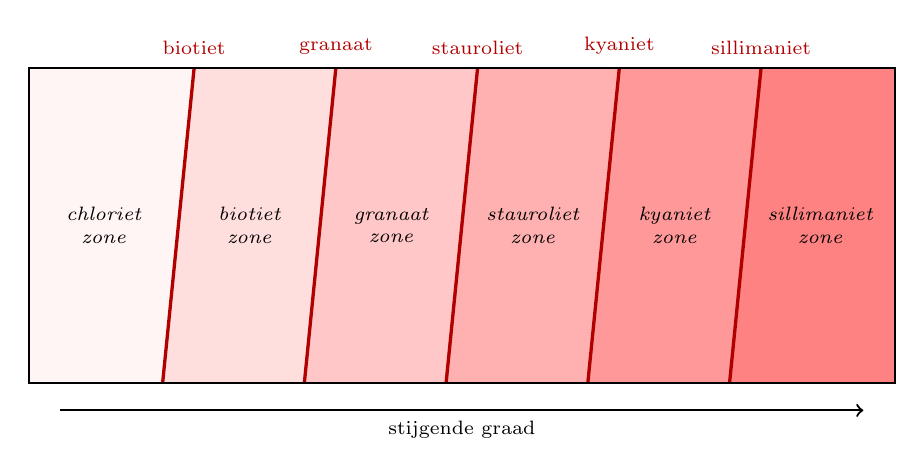
\begin{tikzpicture}[x=1cm, y=1cm]
\def\iso{{0,1.9,3.7,5.5,7.3,9.1,11}}
\foreach \i [evaluate=\i as \op using 4+9*\i] in {0,...,5} {
  \pgfmathsetmacro{\xa}{\iso[\i]}\pgfmathsetmacro{\xb}{\iso[\i+1]}
  \pgfmathsetmacro{\da}{(\i>0)*0.2}\pgfmathsetmacro{\db}{(\i<5)*0.2}
  \fill[red!\op!white] (\xa-\da,0) -- (\xb-\db,0) -- (\xb+\db,4) -- (\xa+\da,4) -- cycle;
}
\foreach \x/\n in {1.9/biotiet, 3.7/granaat, 5.5/stauroliet, 7.3/kyaniet, 9.1/sillimaniet} {
  \draw[very thick, red!70!black] (\x-0.2,0) -- (\x+0.2,4);
  \node[font=\scriptsize, red!70!black, anchor=south] at (\x+0.2,4.05) {\n};
}
\draw[thick] (0,0) rectangle (11,4);
\foreach \x/\z in {0.95/chloriet, 2.8/biotiet, 4.6/granaat, 6.4/stauroliet, 8.2/kyaniet, 10.05/sillimaniet}
  \node[font=\scriptsize\itshape, align=center] at (\x,2) {\z\\zone};
\draw[->, thick] (0.4,-0.35) -- node[below, font=\scriptsize] {stijgende graad} (10.6,-0.35);
\end{tikzpicture}
\par\smallskip{\small \omterm{def:b2:pt-paths:barrovian}{Barrowzones} op een kaart, schematisch. Elke isograad (rode lijn, boven
de kaart benoemd) is de lijn waar zijn indexmineraal voor het eerst verschijnt; de graad, en de diepte van
de kleur, nemen naar rechts toe. Elke zone is genoemd naar het mineraal dat aan haar
lagegraadsgrens verschijnt.}
\end{omfigure}
% ledger: iugs:barrow

Isograden worden gekarteerd uit het verschijnen van mineralen, en worden pas omstandigheden van druk en
temperatuur zodra de reacties erachter bekend zijn. Om verder te gaan moet men
temperatuur en druk in één enkel gesteente meten.

\section{Thermometers en barometers}\label{sec:b2:pt-paths:thermobarometry}

\begin{definition}[Geothermometer; geobarometer; uitwisselingsreactie; netto-overdrachtsreactie]\label{def:b2:pt-paths:thermobarometry}
Een \emph{geothermometer}\index{geothermometer} (\emph{geobarometer}\index{geobarometer}) is
een evenwicht tussen mineralen waarvan de ligging vooral van de temperatuur (de druk) afhangt, zodat
de samenstellingen van de mineralen de temperatuur (de druk) van hun laatste
evenwicht geven. Een \emph{uitwisselingsreactie}\index{uitwisselingsreactie} wisselt twee elementen
uit tussen twee mineralen, zoals ijzer en magnesium tussen granaat en biotiet, zonder
een van beide mineralen te vormen of te vernietigen. Een \emph{netto-overdrachtsreactie}\index{netto-overdrachtsreactie}
maakt sommige mineralen ten koste van andere.
\end{definition}

De meest gebruikte thermometer van \omterm{def:b2:metamorphic-facies:protoliths}{metapelieten} is de uitwisseling van ijzer en magnesium
tussen granaat en biotiet,
\[
\ce{Fe3Al2Si3O12 + KMg3AlSi3O10(OH)2 <=> Mg3Al2Si3O12 + KFe3AlSi3O10(OH)2},
\]
almandien plus flogopiet geeft pyroop plus anniet. Zij $X_{\text{Mg}}$ en $X_{\text{Fe}}$
de fracties van de posities die in elk mineraal door magnesium en ijzer worden ingenomen, en
\[
K_D = \frac{(X_{\text{Mg}}/X_{\text{Fe}})_{\text{granaat}}}{(X_{\text{Mg}}/X_{\text{Fe}})_{\text{biotiet}}}.
\]
% ledger: h97:fs-reaction

\begin{proposition}[Een uitwisselingsevenwicht]\label{prop:b2:pt-paths:exchange}
Als granaat en biotiet ideale oplossingen zijn en $\Delta_r H$, $\Delta_r S$ en $\Delta_r V$ van
de reactie hierboven constant zijn, dan geldt bij evenwicht
\[
3RT\ln K_D = -(\Delta_r H + P\,\Delta_r V) + T\,\Delta_r S,
\qquad\text{dus}\qquad
T = \frac{\Delta_r H + P\,\Delta_r V}{\Delta_r S - 3R\ln K_D}.
\]
\end{proposition}

\begin{proof}
Elk mineraal heeft drie posities voor ijzer of magnesium. In een ideale oplossing is de activiteit van
een eindlid het product van de fracties van de posities die het inneemt: $a_{\text{pyroop}} =
X_{\text{Mg}}^3$ in granaat, enzovoort. De evenwichtsconstante is daarom
\[
K = \frac{a_{\text{pyroop}}\,a_{\text{anniet}}}{a_{\text{almandien}}\,a_{\text{flogopiet}}}
= \frac{X_{\text{Mg,grt}}^3\,X_{\text{Fe,bt}}^3}{X_{\text{Fe,grt}}^3\,X_{\text{Mg,bt}}^3} = K_D^3 .
\]
Bij evenwicht geldt $\Delta_r G^\circ(T, P) + RT\ln K = 0$, met $\Delta_r G^\circ = \Delta_r H -
T\,\Delta_r S + P\,\Delta_r V$ (de 1 van $P - 1$ verwaarloosd), wat de eerste vergelijking geeft;
die naar $T$ oplossen geeft de tweede.
\end{proof}

De constanten komen uit experimenten waarin synthetisch granaat en biotiet ijzer
en magnesium uitwisselden bij bekende temperatuur en \qty{2.07}{kbar}. Twaalf zulke intervallen, van 550 tot
\qty{800}{\celsius}, uitgezet als $\ln K_D$ tegen $1/T$, liggen dicht bij een lijn (de figuur
hieronder); gefit met kleinste kwadraten met $\Delta_r V = \qty{0.311}{J.bar^{-1}}$ geven ze
$\Delta_r H = \qty{52630}{J}$ en $\Delta_r S = \qty{20.19}{J.K^{-1}}$, de waarden van
gepubliceerde herberekeningen van dezelfde gegevens. Bij hogere temperatuur stijgt de verhouding $K_D$
naar 1: granaat neemt een groter deel van het magnesium.
% ledger: h97:fs-data, h97:ideal, h97:fs-reaction

\begin{omfigure}
\centering
\begin{tikzpicture}
\begin{axis}[omrecord, width=0.62\linewidth, height=5.2cm,
  xmin=0.9, xmax=1.25, ymin=-1.9, ymax=-1.1,
  xlabel={$1000/T$ (\unit{K^{-1}})}, ylabel={$\ln K_D$},
  tick label style={font=\scriptsize}, label style={font=\small},
  x tick label style={/pgf/number format/.cd, fixed, precision=2}]
\addplot[only marks, mark=*, mark size=1.6pt, blue!70!black]
  table[x expr={1000/(\thisrow{T_C}+273.15)}, y=lnKD] {figdata/out/bachelor-2-ptpaths-fs.dat};
\addplot[thick, red!75!black, domain=0.9:1.25, samples=2] {(-52630-2070*0.311)/(3*8.31441)*x/1000 + 20.19/(3*8.31441)};
\end{axis}
\end{tikzpicture}
\par\smallskip{\small Uitwisseling granaat--biotiet: de twaalf experimentele intervallen bij
\qty{2.07}{kbar} (blauw, zoals getabelleerd door Holdaway en coauteurs, 1997) en de lijn van
de propositie met de gefitte $\Delta_r H$ en $\Delta_r S$ (rood).}
\end{omfigure}
% ledger: h97:fs-data, h97:ideal

Voor $K_D = 0.18$ bij \qty{5}{kbar} is $T = (52630 + 0.311\times5000)/(20.19 - 3\times8.314
\times\ln 0.18) = 54185/62.96 = \qty{861}{K}$, of \qty{587}{\celsius}. Eén kilobar meer
voegt $0.311\times1000/62.96 = \qty{4.9}{K}$ toe: de reactie wisselt ionen met dezelfde lading
uit tussen posities van bijna dezelfde grootte, haar volumeverandering is klein, en druk doet nauwelijks
ertoe. Dat maakt een thermometer.

Een barometer heeft het omgekeerde nodig: een reactie met een grote volumeverandering. De
\omterm{def:b2:pt-paths:thermobarometry}{netto-overdrachtsreactie}
\[
\ce{3 CaAl2Si2O8 <=> Ca3Al2Si3O12 + 2 Al2SiO5 + SiO2},
\]
anorthiet dat grossulaar, kyaniet en kwarts geeft, pakt de atomen van drie veldspaten in
dichtere mineralen: $\Delta_r V = \qty{-6.21}{J.bar^{-1}}$, twintig keer die van de uitwisseling.
Haar eindlidevenwicht, omgekeerd in experimenten bij 900 tot \qty{1250}{\celsius} en 19
tot \qty{28}{kbar}, loopt langs
\[
P_0 = 22.80\,T - 1093 \qquad (P_0 \text{ in bar}, T \text{ in } \unit{\celsius}).
\]
In een gesteente is grossulaar een klein deel van de granaat en anorthiet een deel van het
plagioklaas. Met ideale activiteiten, $a_{\text{grossulaar}} = X_{\text{Ca,grt}}^3$ en
$a_{\text{anorthiet}} = X_{\text{an}}$, geeft de voorwaarde $\Delta_r G^\circ + RT\ln K = 0$,
geschreven bij $P$ en bij $P_0$,
\[
P = P_0 + \frac{RT}{6.21}\,\ln\frac{X_{\text{Ca,grt}}^3}{X_{\text{an}}^3}
\qquad (T \text{ in kelvin in de tweede term}).
\]
Deze \omterm{def:b2:pt-paths:thermobarometry}{geobarometer}, GASP genoemd naar de Engelse namen van de vier mineralen (granaat, aluminiumsilicaat,
silica, plagioklaas), dient overal waar een \omterm{def:b2:metamorphic-facies:protoliths}{metapeliet} ze alle vier bevat.
% ledger: kn88:gasp, rh95:gb-gasp

\begin{method}[Temperatuur en druk van één gesteente]\label{met:b2:pt-paths:intersection}
(1) Meet, in mineralen die samen groeiden, de samenstellingen die de thermometer en de
barometer nodig hebben. (2) Neem een druk aan en bereken de temperatuur met de thermometer.
(3) Bereken bij die temperatuur de druk met de barometer. (4) Herhaal (2) en (3)
tot geen van beide nog verandert; twee of drie rondes volstaan, omdat elke vergelijking zwak afhangt van
de variabele die de andere vastlegt. Grafisch is het antwoord het punt waar de lijn van de
thermometer de lijn van de barometer snijdt. (5) Plant de onzekerheden voort: voor
onafhankelijke fouten geldt $\sigma_T^2 = (\partial T/\partial\ln K_D)^2\sigma_{\ln K_D}^2 +
(\partial T/\partial P)^2\sigma_P^2$, en evenzo voor $P$.
\end{method}

\begin{omfigure}
\centering
\begin{tikzpicture}
\begin{axis}[omrecord, width=0.78\linewidth, height=6.4cm,
  xmin=400, xmax=800, ymin=0, ymax=12, xlabel={$T$ (\unit{\celsius})}, ylabel={$P$ (\unit{kbar})},
  tick label style={font=\scriptsize}, label style={font=\small}, clip=false]
\addplot[thick, red!75!black] table[x=kd12, y=P_kbar] {figdata/out/bachelor-2-ptpaths-gb.dat};
\addplot[thick, red!75!black] table[x=kd15, y=P_kbar] {figdata/out/bachelor-2-ptpaths-gb.dat};
\addplot[thick, red!75!black] table[x=kd18, y=P_kbar] {figdata/out/bachelor-2-ptpaths-gb.dat};
\addplot[thick, red!75!black] table[x=kd21, y=P_kbar] {figdata/out/bachelor-2-ptpaths-gb.dat};
\addplot[thick, red!75!black] table[x=kd24, y=P_kbar] {figdata/out/bachelor-2-ptpaths-gb.dat};
\addplot[thick, blue!70!black] table[x=T_C, y=r15] {figdata/out/bachelor-2-ptpaths-gasp.dat};
\addplot[thick, blue!70!black] table[x=T_C, y=r20] {figdata/out/bachelor-2-ptpaths-gasp.dat};
\addplot[thick, blue!70!black] table[x=T_C, y=r25] {figdata/out/bachelor-2-ptpaths-gasp.dat};
\addplot[thick, blue!70!black] table[x=T_C, y=r30] {figdata/out/bachelor-2-ptpaths-gasp.dat};
\node[font=\tiny, red!75!black, anchor=west] at (axis cs:452,0.5) {0.12};
\node[font=\tiny, red!75!black, anchor=west] at (axis cs:511,0.5) {0.15};
\node[font=\tiny, red!75!black, anchor=west] at (axis cs:568,0.5) {0.18};
\node[font=\tiny, red!75!black, anchor=west] at (axis cs:622,0.5) {0.21};
\node[font=\tiny, red!75!black, anchor=west] at (axis cs:675,0.5) {0.24};
\node[font=\tiny, blue!70!black, anchor=west] at (axis cs:802,8.97) {0.15};
\node[font=\tiny, blue!70!black, anchor=west] at (axis cs:802,10.21) {0.20};
\node[font=\tiny, blue!70!black, anchor=west] at (axis cs:802,11.17) {0.25};
\node[font=\tiny, blue!70!black, anchor=west] at (axis cs:802,11.96) {0.30};
\end{axis}
\end{tikzpicture}
\par\smallskip{\small Isothermen granaat--biotiet (rood, steil, gelabeld met $K_D$) en
GASP-isobaren (blauw, rechts gelabeld met de verhouding $X_{\text{Ca}}/X_{\text{an}}$ van
grossulaar in granaat tot anorthiet in plagioklaas), uit de kalibraties van deze paragraaf. Een gesteente dat beide paren bevat, ligt
waar zijn twee lijnen elkaar snijden.}
\end{omfigure}
% ledger: h97:ideal, h97:fs-reaction, kn88:gasp

De thermometerlijnen zijn bijna verticaal, de barometerlijnen hellend: ze snijden elkaar onder een
grote hoek, wat het snijpunt precies houdt. Ideale menging is de belangrijkste vereenvoudiging
van dit hoofdstuk. Echte granaten bevatten calcium en mangaan, echte biotieten aluminium,
titaan en ijzer(III), en kalibraties die daarvoor corrigeren, verschuiven temperaturen met
tientallen graden (in een goed bestudeerd gebied \qty{574}{\celsius} in plaats van
\qty{530}{\celsius}); de beste claimen een onzekerheid van ongeveer \qty{25}{\celsius}.
% ledger: h97:ideal, h97:corrections

\section{Druk--temperatuurpaden}\label{sec:b2:pt-paths:paths}

Een gesteente bereikt zijn hoogste druk en zijn hoogste temperatuur niet op hetzelfde moment.
Het wordt begraven en verhit, daarna weer omhooggebracht en afgekoeld, en zijn mineralen reageren de hele
weg door.

\begin{definition}[P--T-pad; prograde en retrograde paden; metamorfe piekomstandigheden]\label{def:b2:pt-paths:paths}
Het \emph{P--T-pad}\index{P--T-pad} van een gesteente is de opeenvolging van drukken en
temperaturen die het tijdens een metamorfe gebeurtenis doorliep. Zijn \emph{prograde
pad}\index{prograde pad} is het deel waarlangs de temperatuur stijgt, zijn \emph{retrograde
pad}\index{retrograde pad} het deel waarlangs ze daalt. De \emph{metamorfe
piekomstandigheden}\index{metamorfe piekomstandigheden} zijn de druk en de temperatuur bij de
hoogste temperatuur van het pad, de thermische piek; de drukpiek, of barische piek, hoeft
er niet mee samen te vallen.
\end{definition}
% ledger: scmr:ptt

Een pad loopt \emph{met de klok mee} wanneer, getekend met de temperatuur naar rechts en de druk omhoog,
de thermische piek na de barische piek komt, tijdens de decompressie; het loopt
\emph{tegen de klok in} wanneer de thermische piek wordt bereikt terwijl de druk nog stijgt. Welke
zin een gesteente volgt, hangt af van hoe de warmte het bereikte, en het eenvoudigste geval laat zich
berekenen.
% ledger: scmr:ptt

Stel een korst voor van \qty{35}{km} dik, in stationaire toestand, met een warmteproductie van
\qty{1.0}{\micro W.m^{-3}}, een warmtestroom van \qty{25}{mW.m^{-2}} van onderen, een geleidbaarheid
van \qty{2.5}{W.m^{-1}.K^{-1}} en een diffusiviteit van \qty{1e-6}{m^2.s^{-1}}, de laatste drie
binnen de bereiken die aan gesteenten zijn gemeten. Haar oppervlaktewarmtestroom is \qty{60}{mW.m^{-2}} en haar Moho ligt op
\qty{595}{\celsius}. Een botsing stapelt een tweede kopie van deze korst erbovenop, snel
vergeleken met de tijd die warmte nodig heeft om zich te verplaatsen: de gesteenten van de onderste plaat houden hun
temperaturen maar zitten \qty{35}{km} dieper, zodat de geotherm een zaagtand wordt, met
gesteenten van \qty{0}{\celsius} op \qty{35}{km} onder hete gesteenten van de bovenste plaat. De korst is
nu \qty{70}{km} dik en bevat tweemaal zoveel warmteproducerend gesteente. Dertig miljoen jaar na
het stapelen begint de erosie, die in 70 miljoen jaar \qty{35}{km} verwijdert
(\qty{0.5}{mm.yr^{-1}}).
% ledger: delaney:conductivity, roy:granitic-k, vila:heat-production, prem:moho-average, et84:ptt

\begin{proposition}[Tijdschaal van thermische relaxatie]\label{prop:b2:pt-paths:relaxation}
In een laag met dikte $L$ waarvan beide vlakken op vaste temperatuur worden gehouden, neemt een
temperatuurverstoring van de vorm $\sin(\pi z/L)$ af als $e^{-t/\tau}$, met
\[
\tau = \frac{L^2}{\pi^2\kappa}.
\]
\end{proposition}

\begin{proof}
Schrijf $\theta(z, t) = f(t)\sin(\pi z/L)$, dat nul is bij $z = 0$ en $z = L$. De
warmtevergelijking $\partial\theta/\partial t = \kappa\,\partial^2\theta/\partial z^2$ geeft
$f'\sin(\pi z/L) = -\kappa(\pi/L)^2 f\sin(\pi z/L)$, dus $f' = -f/\tau$ met $\tau =
L^2/(\pi^2\kappa)$, en $f = f(0)\,e^{-t/\tau}$.
\end{proof}

De zaagtand heeft een golflengte van de orde van de dikte van één plaat: met $L =
\qty{35}{km}$ is $\tau = \qty{3.9}{Myr}$, en de koude wig op \qty{35}{km} is binnen
tien miljoen jaar uitgewist. De hele verdikte korst, $L = \qty{70}{km}$, relaxeert met $\tau =
\qty{16}{Myr}$, zodat de opwarming tientallen miljoenen jaren doorgaat, naar de veel
hetere geotherm die een korst van dubbele dikte en met tweemaal zoveel warmteproducerend gesteente
onderhoudt. De figuur
hieronder toont de berekende geothermen.
% ledger: delaney:conductivity

\begin{omfigure}
\centering
\begin{tikzpicture}
\begin{axis}[omrecord, width=0.62\linewidth, height=6.6cm,
  xmin=0, xmax=1000, ymin=0, ymax=80, y dir=reverse,
  xlabel={$T$ (\unit{\celsius})}, ylabel={diepte (\unit{km})},
  legend style={font=\scriptsize, at={(0.02,0.02)}, anchor=south west},
  tick label style={font=\scriptsize}, label style={font=\small}]
\addplot[thick, black] table[x=t0, y=z_km] {figdata/out/bachelor-2-ptpaths-geo.dat};
\addlegendentry{\qty{0}{Myr}}
\addplot[thick, blue!70!black] table[x=t10, y=z_km] {figdata/out/bachelor-2-ptpaths-geo.dat};
\addlegendentry{\qty{10}{Myr}}
\addplot[thick, orange!85!black] table[x=t30, y=z_km] {figdata/out/bachelor-2-ptpaths-geo.dat};
\addlegendentry{\qty{30}{Myr}}
\addplot[thick, red!75!black] table[x=t60, y=z_km] {figdata/out/bachelor-2-ptpaths-geo.dat};
\addlegendentry{\qty{60}{Myr}}
\end{axis}
\end{tikzpicture}
\par\smallskip{\small Geothermen na het verdubbelen van een korst van \qty{35}{km} door stapeling, berekend
met de warmtevergelijking (diepten onder het oppervlak van dat moment; de erosie begint bij
\qty{30}{Myr}). Zwart: de zaagtand net na het stapelen. De basis van de verdikte korst,
eerst op \qty{595}{\celsius}, passeert \qty{900}{\celsius} na 60 miljoen jaar.}
\end{omfigure}
% ledger: et84:ptt

Volg het gesteente dat vóór het stapelen aan het oppervlak lag en er net na op \qty{35}{km}
ligt, onder \qty{9.6}{kbar}. In vijf miljoen jaar warmt het op van 0 tot
\qty{395}{\celsius} zonder te bewegen; bij het begin van de erosie heeft het
\qty{558}{\celsius} bereikt. De erosie brengt het dan omhoog, maar warmte komt sneller aan dan ze
ontsnapt: het gesteente warmt nog op wanneer het \qty{6}{km} is gestegen, en bereikt zijn thermische
piek, \qty{593}{\celsius} bij \qty{7.8}{kbar}, 43 miljoen jaar na het stapelen. Pas
dan koelt het af, via \qty{405}{\celsius} op \qty{13}{km} diepte en
\qty{74}{Myr}, op weg naar het oppervlak. Het pad (de figuur hieronder) loopt met de klok mee. Het blijft
ook dertig miljoen jaar binnen \qty{50}{\celsius} van zijn piektemperatuur, ongeveer een
derde van zijn hele tocht, zoals England en Thompson in 1984 vonden voor de meeste geologisch
plausibele gevallen: een gesteente verblijft lang dicht bij zijn piek, en de mineralen die het bewaart,
leggen vooral dat stadium vast.
% ledger: et84:ptt

\begin{omfigure}
\centering
\begin{tikzpicture}
\begin{axis}[omrecord, width=0.78\linewidth, height=6.2cm,
  xmin=0, xmax=800, ymin=0, ymax=11, xlabel={$T$ (\unit{\celsius})}, ylabel={$P$ (\unit{kbar})},
  tick label style={font=\scriptsize}, label style={font=\small}]
\addplot[thick, gray, densely dashed, restrict x to domain=0:504] table[x=T_C, y=P_kbar] {figdata/out/bachelor-2-facies-hm93-kyand.dat};
\addplot[thick, gray, densely dashed] table[x=T_C, y=P_kbar] {figdata/out/bachelor-2-facies-hm93-kysil.dat};
\addplot[thick, gray, densely dashed] table[x=T_C, y=P_kbar] {figdata/out/bachelor-2-facies-hm93-andsil.dat};
\addplot[very thick, red!75!black, postaction={decorate}, decoration={markings,
  mark=at position 0.2 with {\arrow{Stealth[length=2.5mm]}},
  mark=at position 0.52 with {\arrow{Stealth[length=2.5mm]}},
  mark=at position 0.8 with {\arrow{Stealth[length=2.5mm]}}}] table[x=T_C, y=P_kbar] {figdata/out/bachelor-2-ptpaths-path.dat};
\node[font=\scriptsize\bfseries, gray] at (axis cs:330,6.5) {kyaniet};
\node[font=\scriptsize\bfseries, gray] at (axis cs:520,1.0) {andalusiet};
\node[font=\scriptsize\bfseries, gray] at (axis cs:740,4.0) {sillimaniet};
\node[font=\scriptsize, red!75!black, anchor=south] at (axis cs:200,9.7) {opwarming in de diepte};
\node[font=\scriptsize, red!75!black, anchor=west] at (axis cs:603,8.9) {thermische piek};
\node[font=\scriptsize, red!75!black, anchor=west] at (axis cs:110,2.7) {afkoelend opstijgen};
\end{axis}
\end{tikzpicture}
\par\smallskip{\small \omterm{def:b2:pt-paths:paths}{P--T-pad} van het gesteente dat net na het stapelen op \qty{35}{km} ligt
(rood, om de twee miljoen jaar bemonsterd), berekend met het model van de geothermen hierboven,
over het experimentele \ce{Al2SiO5}-diagram van \cref{ch:b2:metamorphic-facies} (grijs). De
drukpiek komt eerst, de thermische piek tijdens de decompressie: een pad met de klok mee, dat
het kyanietveld nooit verlaat.}
\end{omfigure}
% ledger: et84:ptt, hm93:table11

Het model toont ook waarom sommige paden de andere kant op draaien. Verdikking alleen verhit een gesteente
pas nadat het is begraven, dus zijn thermische piek komt tijdens de \omterm{def:b2:pt-paths:exhumation}{exhumatie}. Een gesteente waarvan
de temperatuur stijgt terwijl het nog wordt begraven, heeft warmte van elders nodig, zoals \omterm{def:b2:magma-emplacement:magma}{magma}
dat in de korst erboven of ernaast opstijgt, en volgt een pad tegen de klok in. En in de
verdikte korst wordt de basis veel heter dan haar begintemperatuur: England en Thompson
concludeerden dat aanzienlijk smelten van de korst een waarschijnlijk gevolg van verdikking is,
het onderwerp van \cref{ch:b2:crustal-melting}.
% ledger: et84:ptt, scmr:ptt

\section{De tijd toevoegen}\label{sec:b2:pt-paths:time}

\begin{definition}[P--T--t-pad]\label{def:b2:pt-paths:ptt}
Het \emph{P--T--t-pad}\index{P--T--t-pad} van een gesteente is zijn \omterm{def:b2:pt-paths:paths}{P--T-pad} met het tijdstip
waarop elk punt werd bereikt.
\end{definition}
% ledger: scmr:ptt

De tijd komt uit radiometrische datering. Een mineraal dat tijdens de gebeurtenis groeide en sindsdien
zijn dochterisotopen heeft behouden, zoals een granaatzone gedateerd met de
samarium--neodymiummethode, dateert zijn eigen groei, en zijn
samenstelling geeft de druk en de temperatuur van dat moment. Een mineraal dat
eerder groeide, bij hogere temperatuur, geeft in plaats daarvan een afkoelingsouderdom: het tijdstip waarop het gesteente
afkoelde door de sluitingstemperatuur van dat mineraal en isotopensysteem
(Boek~3). Voor argon in een muscovietkorrel met een straal van \qty{100}{\micro m}, die afkoelt met
\qty{10}{\celsius} per miljoen jaar, is de sluitingstemperatuur \qty{405}{\celsius} bij
\qty{5}{kbar} en \qty{425}{\celsius} bij \qty{10}{kbar}.
% ledger: h09:muscovite

\begin{definition}[Exhumatie; exhumatiesnelheid]\label{def:b2:pt-paths:exhumation}
\emph{Exhumatie}\index{exhumatie} is de beweging van een gesteente naar het aardoppervlak,
door verwijdering van de gesteenten erboven. De \emph{exhumatiesnelheid}\index{exhumatiesnelheid} is de
snelheid waarmee zijn diepte afneemt.
\end{definition}

\begin{proposition}[Snelheden uit twee gedateerde punten]\label{prop:b2:pt-paths:rates}
Als een gesteente temperatuur $T_1$ en diepte $z_1$ had op tijdstip $t_1$, en $T_2$, $z_2$ op een
later tijdstip $t_2$ (ouderdommen teruggeteld vanaf nu, $t_1 > t_2$), dan zijn zijn gemiddelde afkoelings- en
\omterm{def:b2:pt-paths:exhumation}{exhumatiesnelheid} over het interval
\[
\frac{T_1 - T_2}{t_1 - t_2}
\qquad\text{en}\qquad
\frac{z_1 - z_2}{t_1 - t_2},
\]
en volgen hun onzekerheden, voor onafhankelijke fouten op de twee ouderdommen, uit
$\sigma_{t_1 - t_2}^2 = \sigma_{t_1}^2 + \sigma_{t_2}^2$.
\end{proposition}

\begin{proof}
Een gemiddelde snelheid is een verschil gedeeld door de verstreken tijd $t_1 - t_2$; de variantie van een
verschil van onafhankelijke grootheden is de som van hun varianties.
\end{proof}

De diepte waarop een afkoelingsouderdom werd vastgelegd, wordt zelden gemeten: ze wordt geschat uit de
geotherm van dat moment, en daarom zijn exhumatiesnelheden onzekerder dan afkoelingssnelheden.
Een druk, waar een \omterm{def:b2:metamorphic-facies:assemblage}{minerale associatie} er een geeft, legt de diepte rechtstreeks vast, als
$z = P/(\bar\rho g)$ met $\bar\rho$ de gemiddelde dichtheid van de gesteenten erboven.

\section{Metamorfe reeksen en gepaarde gordels}\label{sec:b2:pt-paths:series}

\begin{definition}[Metamorfe reeks; gepaarde metamorfe gordels]\label{def:b2:pt-paths:series}
Een \emph{metamorfe reeks}\index{metamorfe reeks} (of faciesreeks) is een opeenvolging van
\omterm{def:b2:metamorphic-facies:facies}{metamorfe facies} die zich ontwikkelt onder hetzelfde bereik van verhoudingen van druk tot temperatuur,
en die daardoor een radiale sector van het druk--temperatuurvlak inneemt.
\emph{Gepaarde metamorfe gordels}\index{gepaarde metamorfe gordels} zijn twee evenwijdige gordels van
dezelfde ouderdom, een met een hogedrukreeks en een met een lagedrukreeks.
\end{definition}
% ledger: scmr:ptt, wallis24:paired

Gewoonlijk worden drie reeksen onderscheiden. Een hoge verhouding van druk tot temperatuur, langs een
koude gradiënt, leidt van de zeolietfacies naar de blauwschisten en eclogieten: de reeks
van subductiezones. Een gemiddelde verhouding leidt door de groenschist-, amfiboliet- en
granulietfacies, met kyaniet en daarna sillimaniet in \omterm{def:b2:metamorphic-facies:protoliths}{metapelieten}: de Barrowreeks. Een lage
verhouding, langs hete gradiënten zoals die bij intrusies, levert andalusiet en daarna
sillimaniet op: de lagedruk- of Buchanreeks. De figuur hieronder tekent drie gradiënten
over het aluminiumsilicaatdiagram.
% ledger: scmr:ptt, scmr:facies, iugs:barrow, fub:paired

\begin{omfigure}
\centering
\begin{tikzpicture}
\begin{axis}[omrecord, width=0.78\linewidth, height=6.2cm,
  xmin=0, xmax=900, ymin=0, ymax=12, xlabel={$T$ (\unit{\celsius})}, ylabel={$P$ (\unit{kbar})},
  tick label style={font=\scriptsize}, label style={font=\small}]
\addplot[thick, gray, densely dashed, restrict x to domain=0:504] table[x=T_C, y=P_kbar] {figdata/out/bachelor-2-facies-hm93-kyand.dat};
\addplot[thick, gray, densely dashed] table[x=T_C, y=P_kbar] {figdata/out/bachelor-2-facies-hm93-kysil.dat};
\addplot[thick, gray, densely dashed] table[x=T_C, y=P_kbar] {figdata/out/bachelor-2-facies-hm93-andsil.dat};
\addplot[very thick, blue!70!black] table[x=T_C, y=g10] {figdata/out/bachelor-2-ptpaths-series.dat};
\addplot[very thick, green!45!black] table[x=T_C, y=g25] {figdata/out/bachelor-2-ptpaths-series.dat};
\addplot[very thick, orange!85!black] table[x=T_C, y=g60] {figdata/out/bachelor-2-ptpaths-series.dat};
\node[font=\scriptsize, blue!70!black, rotate=52, anchor=south] at (axis cs:330,8.5) {\qty{10}{\celsius\per\km}};
\node[font=\scriptsize, green!45!black, rotate=28, anchor=south] at (axis cs:640,7.0) {\qty{25}{\celsius\per\km}};
\node[font=\scriptsize, orange!85!black, rotate=12, anchor=south] at (axis cs:800,3.65) {\qty{60}{\celsius\per\km}};
\node[font=\scriptsize\bfseries, gray] at (axis cs:120,5.5) {kyaniet};
\node[font=\scriptsize\bfseries, gray] at (axis cs:470,1.1) {andalusiet};
\node[font=\scriptsize\bfseries, gray] at (axis cs:800,1.6) {sillimaniet};
\end{axis}
\end{tikzpicture}
\par\smallskip{\small Drie geothermische gradiënten vanaf een oppervlak van \qty{10}{\celsius},
omgerekend naar druk met een gemiddelde dichtheid van \qty{2800}{kg.m^{-3}}, over het experimentele
\ce{Al2SiO5}-diagram (grijs). De koude gradiënt blijft in het kyanietveld, de
gemiddelde gaat van kyaniet naar sillimaniet, de hete doorkruist het
andalusietveld voordat hij sillimaniet bereikt.}
\end{omfigure}
% ledger: hm93:table11

Het idee van de reeksen kwam uit Japan, waar Akiho Miyashiro ze in 1961 definieerde. In
het zuidwesten van het land loopt de Sanbagawagordel, met hogedruk-,
lagetemperatuurmetamorfose, over meer dan \qty{800}{km} naast de Ryokegordel, met hogetemperatuur-,
lagedrukmetamorfose, gescheiden door een grote breuk: het klassieke paar. De
Sanbagawagordel is een oude subductiezone, de Ryokegordel de vulkanische boog erboven. Een
subductiezone maakt dus beide reeksen tegelijk, koude gesteenten die door de zinkende
plaat omlaag worden gesleept, hete die in de boog worden verhit; gepaarde gordels van dezelfde soort zijn bekend rond de
Stille Oceaan.
% ledger: wallis24:paired, koguchi17:paired, fub:paired, scmr:ptt

\section{Ultrahoge druk en exhumatie}\label{sec:b2:pt-paths:uhp}

In 1984 werd uit het Dora-Mairamassief in de westelijke
Alpen een kwartsiet beschreven waarvan de granaten, tot \qty{25}{cm} groot en bijna zuiver pyroop, korrels
coësiet insluiten, de dichte polymorf van silica, gedeeltelijk weer omgezet in kwarts; de uitzetting
tijdens die omzetting deed de omringende granaat radiaal rond elke korrel barsten. Het coësiet en
zijn begeleiders vereisen minstens \qty{28}{kbar} bij ongeveer \qty{700}{\celsius}: gesteenten van de
bovenste continentale korst, ooit sedimenten, waren tot \qty{90}{km} of dieper afgedaald en weer
teruggekomen.
% ledger: chopin84:coesite

\begin{definition}[Ultrahogedrukmetamorfose]\label{def:b2:pt-paths:uhp}
\emph{Ultrahogedrukmetamorfose}\index{ultrahogedrukmetamorfose} is
\omterm{def:b2:metamorphic-facies:metamorphism}{metamorfose} van korstgesteenten bij drukken die hoog genoeg zijn om coësiet, of diamant, te laten groeien.
\end{definition}

\begin{omfigure}
\centering
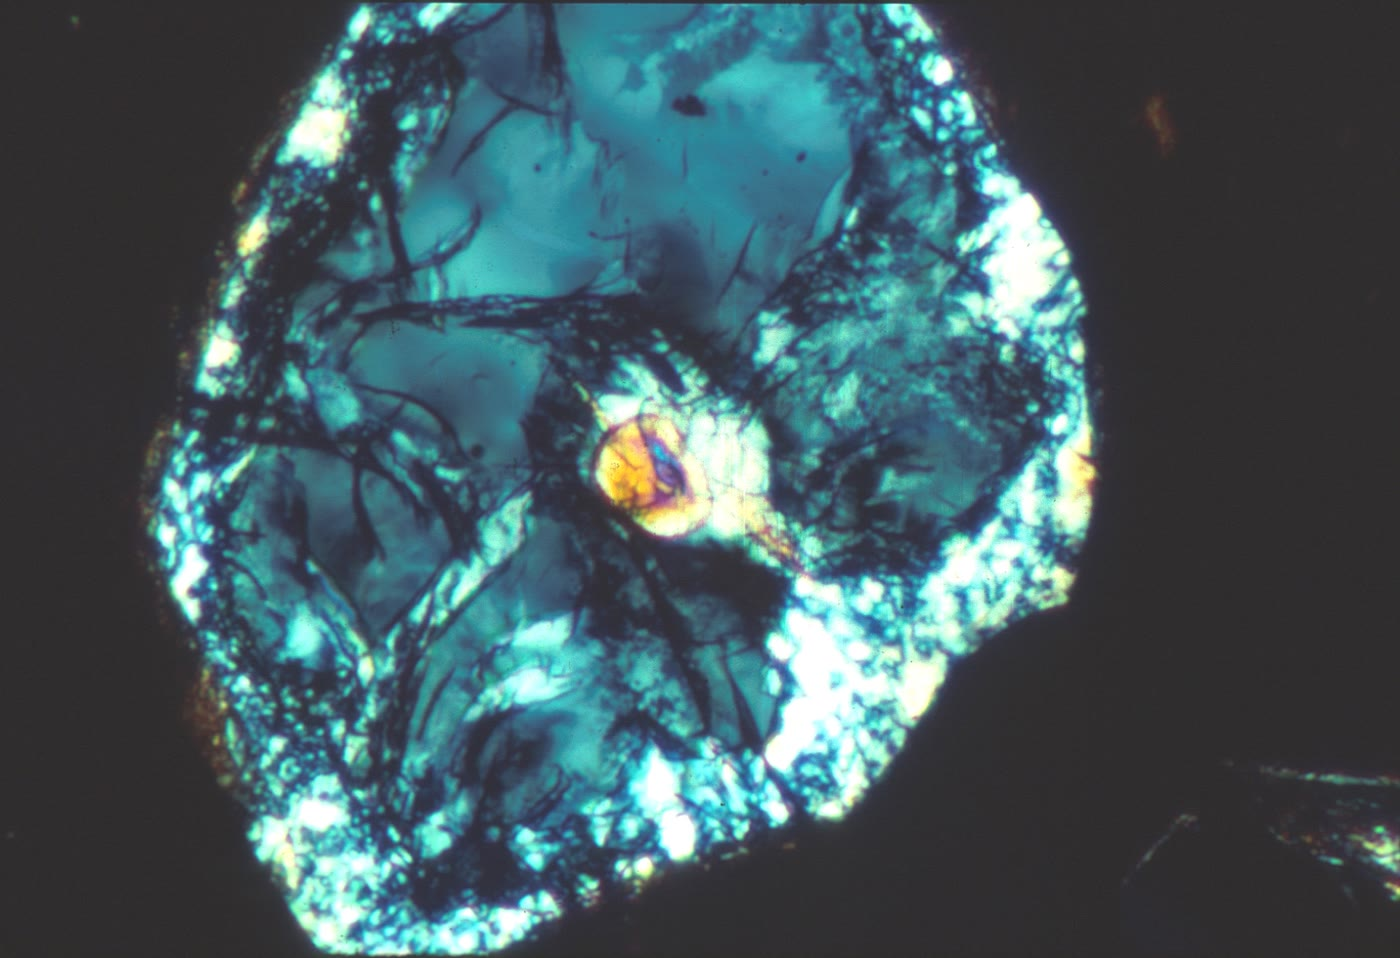
\includegraphics[width=0.62\linewidth]{images/book4/b2-11-coesite.jpg}
\par\smallskip{\small Coësiet in een eclogiet, ongeveer \qty{1}{mm} groot, in een slijpplaatje
tussen gekruiste polarisatoren: de grote centrale korrel is coësiet, de rand van kleine heldere korrels is
kwarts dat eruit groeide toen de druk daalde; de kleine gekleurde korrel in het midden is een
pyroxeeninsluitsel. Foto J.\,R. Smyth, CC BY-SA 1.0.}
\end{omfigure}

Zes jaar later werden diamanten van gemiddeld \qty{12}{\micro m} gevonden in gneisen, schisten en
granaat--pyroxeengesteenten van het Kokchetavmassief in het noorden van Kazachstan, ingesloten in granaat
en zirkoon, die ze ervoor behoedden in grafiet over te gaan: ze groeiden bij \qty{40}{kbar}
of meer en boven 900 tot \qty{1000}{\celsius}. Continentale korst, hoe licht ook, kan
meer dan honderd kilometer omlaag worden gesleept.
% ledger: ss90:diamond

Hoe ze terugkomt, vertellen haar klokken. In de diepst gesubduceerde gesteenten van de Alpen
toont titaniet, gedateerd in opeenvolgende stadia, dat een kalksilicaatgesteente ongeveer
\qty{3.5}{GPa} bereikte op $35.1 \pm \qty{0.9}{Ma}$, op $1 \pm \qty{0.15}{GPa}$ zat op $32.9 \pm
\qty{0.9}{Ma}$, en bij 0.4 tot \qty{0.5}{GPa} op $31.8 \pm \qty{0.5}{Ma}$. De gemiddelde
exhumatiesnelheden, 3.4 en daarna \qty{1.6}{cm.yr^{-1}}, komen overeen met de snelheden van platen: de gesteenten
kwamen ongeveer even snel terug als ze waren afgedaald, veel sneller dan erosie ze had kunnen
blootleggen. De auteurs beroepen zich op het drijfvermogen, de lichte korst die door de dichtere mantel opstijgt, en op
afschuivingsbreuken, die de gesteenten erboven dunner maken.
% ledger: rh01:exhumation

\section{Oceaanbodemmetamorfose}\label{sec:b2:pt-paths:ocean-floor}

\begin{definition}[Oceaanbodemmetamorfose; serpentinisatie]\label{def:b2:pt-paths:ocean-floor}
\emph{Oceaanbodemmetamorfose}\index{oceaanbodemmetamorfose} is de regionale
\omterm{def:b2:metamorphic-facies:metamorphism}{metamorfose} van de oceanische lithosfeer bij spreidingscentra, door hete waterige fluïda
die onder steile geothermische gradiënten circuleren; de herkristallisatie is meestal onvolledig
en de temperatuur neemt typisch toe met de diepte. \emph{Serpentinisatie}\index{serpentinisatie}
is de hydratatie van olivijnrijke gesteenten tot serpentijn.
\end{definition}
% ledger: scmr:types

Zeewater dat bij een rugas in de jonge korst wordt gezogen, warmt op, reageert met de gesteenten en
stijgt weer op. De basalten die het doorstroomt, herkristalliseren, onvolledig, tot waterhoudende
mineralen, over een breed temperatuurbereik. Waar het water \omterm{def:b2:mantle-melting:peridotites}{peridotiet} bereikt, zoals bij
de trage ruggen waar mantelgesteente tot aan de zeebodem opkomt en bronnen voedt zoals
die van het veld Lost City (Boek~3), neemt olivijn water op:
\[
\ce{2 Mg2SiO4 + 3 H2O -> Mg3Si2O5(OH)4 + Mg(OH)2},
\]
forsteriet dat serpentijn en bruciet geeft. De molaire volumes, 43.65 voor forsteriet, 107.50
voor serpentijn en \qty{24.63}{cm^3.mol^{-1}} voor bruciet, tonen wat dit met het gesteente doet:
\qty{87.30}{cm^3} olivijn wordt \qty{132.13}{cm^3} vaste stof, \qty{51}{\percent}
meer, en de dichtheid daalt van 3.22 tot \qty{2.54}{g.cm^{-3}}. Het gesteente zwelt op en
wordt lichter, en het water dat het heeft gebonden, gaat met het mee omlaag wanneer de plaat subduceert.
% ledger: scmr:types, rh95:serpentine, kelley:lost-city, dick:ultraslow

\begin{inthelab}[Een granaat lezen]
Om een \omterm{def:b2:pt-paths:paths}{P--T-pad} te lezen, snijdt een petroloog eerst een slijpplaatje door het midden van een
granaat, omdat een doorsnede buiten het midden de kern mist. Onder de microscoop worden de insluitsels
in kaart gebracht: kleine korrels kwarts, biotiet, plagioklaas of kyaniet die werden ingesloten terwijl de granaat
groeide, soms gerangschikt in sporen die een oudere foliatie van het gesteente bewaren. Een
elektronenmicrosonde meet daarna de samenstelling langs een lijn van kern naar rand, en een kaart van
magnesium, ijzer, calcium en mangaan toont de groeizones. Elke zone wordt gekoppeld aan
de mineralen die ermee groeiden: insluitsels voor de kern, de matrix in contact voor de
rand. Thermometer en barometer worden op elk paar toegepast, en de zones worden gedateerd waar een
mineraal dat toelaat. \Cref{ch:b2:field-lab-methods-2} beschrijft de instrumenten.
\end{inthelab}

\begin{omfigure}
\centering
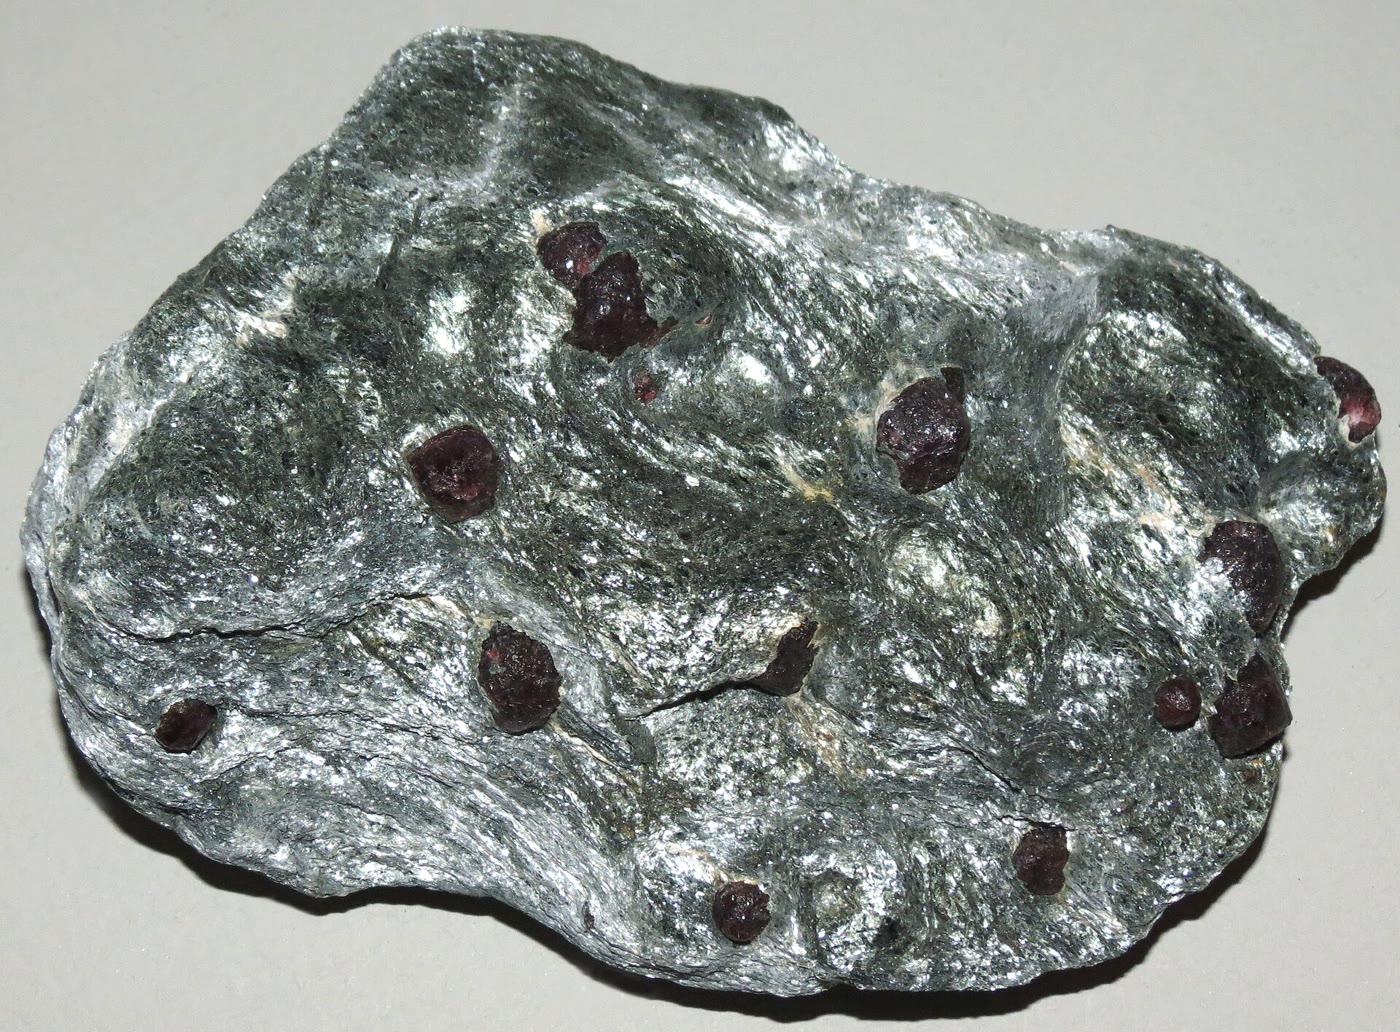
\includegraphics[width=0.62\linewidth]{images/book4/b2-11-garnet-schist.jpg}
\par\smallskip{\small Een granaatschist: donkerrode granaatkristallen gegroeid in een gefolieerde
matrix van mica's. Elke granaat kan, van kern tot rand, een
verslag van het pad van het gesteente bevatten. Foto James St.~John, CC BY 2.0.}
\end{omfigure}

\section{Oefeningen}

\begin{exercise}[$\star$]\label{exo:b2:pt-paths:1}
Zes monsters uit één kleisteenformatie, verzameld langs een weg, bevatten: (A) chloriet,
muscoviet, kwarts; (B) biotiet, chloriet, muscoviet, kwarts; (C) granaat, biotiet,
muscoviet, kwarts; (D) stauroliet, granaat, biotiet, muscoviet, kwarts; (E) kyaniet,
stauroliet, biotiet, muscoviet, kwarts; (F) sillimaniet, biotiet, muscoviet, kwarts.
(a) Bepaal in welke Barrowzone elk ligt. (b) Bepaal hoeveel isograden de weg kruist, en
welke. (c) Waarom volstaat het niet de isograden te kennen om de \omterm{def:b2:pt-paths:barrovian}{metamorfe
veldgradiënt} te tekenen?
\end{exercise}
% ledger: iugs:barrow

\begin{exercise}[$\star$]\label{exo:b2:pt-paths:2}
Een granaat heeft $X_{\text{Mg}} = 0.10$ en $X_{\text{Fe}} = 0.80$, het biotiet ernaast
$X_{\text{Mg}} = 0.45$ en $X_{\text{Fe}} = 0.50$. (a) Bereken $K_D$ en $\ln K_D$.
(b) Bereken met de kalibratie van dit hoofdstuk de temperatuur bij \qty{5}{kbar} en bij
\qty{7}{kbar}. (c) Is het resultaat een temperatuur- of een drukmeter?
\end{exercise}
% ledger: h97:ideal, h97:fs-reaction

\begin{exercise}[$\star$]\label{exo:b2:pt-paths:3}
Een \omterm{def:b2:metamorphic-facies:protoliths}{metapeliet} geeft \qty{580}{\celsius} en \qty{6.0}{kbar}. (a) Bepaal hoe diep hij lag onder gesteenten met een gemiddelde
dichtheid van \qty{2800}{kg.m^{-3}} ($g = \qty{9.81}{m.s^{-2}}$). (b) Bepaal welke
temperatuurgradiënt dat inhoudt vanaf \qty{10}{\celsius} aan het oppervlak. (c) De
experimentele lijn kyaniet $=$ sillimaniet gaat door \qty{3.67}{kbar} bij
\qty{500}{\celsius} en \qty{5.77}{kbar} bij \qty{600}{\celsius}: welk aluminiumsilicaat
zou het gesteente moeten bevatten?
\end{exercise}
% ledger: hm93:table11

\begin{exercise}[$\star$]\label{exo:b2:pt-paths:4}
Voor de \omterm{def:b2:pt-paths:ocean-floor}{serpentinisatie} van forsteriet zoals in dit hoofdstuk geschreven: (a) ga na dat de
vergelijking in massa klopt, met molaire massa's 140.693 (forsteriet), 18.015 (water),
277.112 (serpentijn) en \qty{58.320}{g.mol^{-1}} (bruciet); (b) bereken de verandering van het
volume van de vaste stoffen; (c) bereken de dichtheden van het olivijn en van de producten.
(d) Wat doet de verandering met een geserpentiniseerde \omterm{def:b2:mantle-melting:peridotites}{peridotiet} onder de zeebodem?
\end{exercise}
% ledger: rh95:serpentine

\begin{exercise}[$\star\star$]\label{exo:b2:pt-paths:5}
Kalibreer de thermometer uit vier van de experimenten bij \qty{2.07}{kbar}: $\ln K_D =
-1.157$ en $-1.255$ bij \qty{799}{\celsius}, $-1.738$ en $-1.826$ bij \qty{550}{\celsius}.
(a) Middel elk paar en bepaal de lijn $\ln K_D = a/T + b$ door de twee gemiddelden.
(b) Leid $\Delta_r H$ en $\Delta_r S$ af, met $\Delta_r V = \qty{0.311}{J.bar^{-1}}$.
(c) Vergelijk de temperaturen die de eigen kalibratie en die van het hoofdstuk geven bij
\qty{5}{kbar} voor $K_D = 0.18$, $0.10$ en $0.30$. Wat volgt daaruit over het
extrapoleren van een kalibratie?
\end{exercise}
% ledger: h97:fs-data, h97:ideal

\begin{exercise}[$\star\star$]\label{exo:b2:pt-paths:6}
(a) Bereken uit de molaire volumes bij \qty{298}{K} (almandien 115.32, pyroop 113.12, anniet
154.30, flogopiet 149.65, grossulaar 125.28, anorthiet 100.79, kyaniet 44.15, kwarts
\qty{22.69}{cm^3.mol^{-1}}) $\Delta_r V$ van de uitwisseling en van de GASP-reactie,
en vergelijk met de waarden die de kalibraties gebruiken, \num{0.311} en
\qty{-6.21}{J.bar^{-1}}. (b) Bepaal voor $K_D = 0.18$ met hoeveel kelvin een fout van
\qty{1}{kbar} de temperatuur verschuift. (c) Bepaal langs de GASP-lijn van een gesteente met
$X_{\text{Ca}}/X_{\text{an}} = 0.20$ met hoeveel bar een fout van \qty{17}{K} de
druk verschuift.
\end{exercise}
% ledger: rh95:gb-gasp, rh95:al2sio5, h97:fs-reaction, kn88:gasp

\begin{exercise}[$\star\star$]\label{exo:b2:pt-paths:7}
Bij \qty{600}{\celsius} heeft een granaat $X_{\text{Ca}} = 0.08$ en het plagioklaas ernaast
$X_{\text{an}} = 0.30$. (a) Bereken de GASP-druk. (b) Herhaal met $X_{\text{an}} =
0.35$. (c) Bepaal hoe diep het gesteente lag, bij een gemiddelde dichtheid van \qty{2800}{kg.m^{-3}}.
\end{exercise}
% ledger: kn88:gasp

\begin{exercise}[$\star\star$]\label{exo:b2:pt-paths:8}
Gebruik de titanietouderdommen van de diepst gesubduceerde gesteenten van de Alpen: ongeveer \qty{3.5}{GPa} op
$35.1 \pm \qty{0.9}{Ma}$, \qty{1.0}{GPa} op $32.9 \pm \qty{0.9}{Ma}$, \qty{0.45}{GPa} op
$31.8 \pm \qty{0.5}{Ma}$. (a) Reken de drukken met een gemiddelde dichtheid van \qty{3000}{kg.m^{-3}} om
naar diepten. (b) Bereken de twee gemiddelde exhumatiesnelheden en vergelijk met de
gepubliceerde 3.4 en \qty{1.6}{cm.yr^{-1}}. (c) Bepaal de onzekerheid van het eerste
tijdsinterval, en welk bereik van snelheden ze toelaat. (d) Vergelijk met de erosiesnelheid van
het verdikkingsmodel, \qty{0.5}{mm.yr^{-1}}.
\end{exercise}
% ledger: rh01:exhumation

\begin{exercise}[$\star\star$]\label{exo:b2:pt-paths:9}
Voor $K_D = 0.18$ bij \qty{5}{kbar}: (a) bereken $\partial T/\partial\ln K_D$ en
$\partial T/\partial P$ uit de propositie; (b) bereken met $\sigma_{\ln K_D} = 0.05$ (een
fout van \qty{5}{\percent} op $K_D$) en $\sigma_P = \qty{1}{kbar}$ de waarde $\sigma_T$.
(c) Welke fout overheerst? Vergelijk met de onzekerheid van \qty{25}{\celsius} die voor
de beste kalibraties wordt geclaimd.
\end{exercise}
% ledger: h97:ideal

\begin{exercise}[$\star\star\star$]\label{exo:b2:pt-paths:10}
Een granaatrand heeft $X_{\text{Mg}} = 0.10$, $X_{\text{Fe}} = 0.75$, $X_{\text{Ca}} = 0.07$;
het matrixbiotiet $X_{\text{Mg}} = 0.42$, $X_{\text{Fe}} = 0.52$; het plagioklaas
$X_{\text{an}} = 0.25$. (a) Pas de methode van dit hoofdstuk toe, beginnend bij \qty{6}{kbar},
tot de temperatuur met minder dan \qty{1}{K} verandert. (b) Bepaal welk aluminiumsilicaat
het gesteente zou moeten bevatten (gebruik de experimentele lijn van \cref{exo:b2:pt-paths:3}). (c) Waarom moet de barometer
het werkelijk aanwezige aluminiumsilicaat gebruiken?
\end{exercise}
% ledger: h97:ideal, kn88:gasp, hm93:table11

\begin{exercise}[$\star\star\star$]\label{exo:b2:pt-paths:11}
Met $\kappa = \qty{1e-6}{m^2.s^{-1}}$: (a) bereken de relaxatietijd van de
propositie voor $L = \qty{35}{km}$ en voor $L = \qty{70}{km}$. (b) Het model erodeert
\qty{35}{km} in 70 miljoen jaar; vergelijk die tijd met de twee van (a). (c) Verklaar
uit deze tijden waarom het gesteente van het model zijn thermische piek na zijn
drukpiek bereikt. (d) Wat zou er in het pad veranderen als de erosie tien keer sneller was?
\end{exercise}
% ledger: delaney:conductivity, et84:ptt

\begin{exercise}[$\star\star\star$]\label{exo:b2:pt-paths:12}
Neem een korst van \qty{35}{km} dik met dichtheid \qty{2800}{kg.m^{-3}} boven een mantel van
\qty{3300}{kg.m^{-3}}. (a) Bepaal op welke diepte de druk \qty{28}{kbar} bereikt, het
minimum voor het coësiet van Dora Maira. (b) En \qty{40}{kbar}, voor de diamanten van Kokchetav?
(c) Bepaal welke gemiddelde gradiënt \qty{700}{\celsius} op de diepte van (a) inhoudt, en in welke
reeks die valt. (d) Bepaal hoe lang de klim van de diepte
van (a) tot \qty{35}{km} duurt bij \qty{3.4}{cm.yr^{-1}}.
\end{exercise}
% ledger: chopin84:coesite, ss90:diamond, rh01:exhumation

\section{Probleem: De reis van een granaat}

\begin{problem}[{Weekendprobleem --- thermobarometrie, pad en exhumatiesnelheid van één
schist}]
\label{pb:b2:pt-paths:1}
Een kyaniet--granaat--biotietschist bevat granaten met een kern en een rand. De kern sluit
biotiet, plagioklaas en kyaniet in; de rand raakt het biotiet en plagioklaas van de
matrix. Rond de granaten is wat kyaniet vervangen door sillimaniet, en aan de randen van
de granaten is wat chloriet gegroeid. De analyses zijn:
\begin{center}
\small
\begin{tabular}{@{}lccc@{}}
\hline
 & $X_{\text{Mg}}$ & $X_{\text{Fe}}$ & $X_{\text{Ca}}$ of $X_{\text{an}}$\\
\hline
granaatkern & 0.080 & 0.760 & 0.050\\
biotiet ingesloten in de kern & 0.40 & 0.58 & ---\\
plagioklaas ingesloten in de kern & --- & --- & 0.25\\
granaatrand & 0.120 & 0.720 & 0.060\\
matrixbiotiet & 0.46 & 0.53 & ---\\
matrixplagioklaas & --- & --- & 0.28\\
\hline
\end{tabular}
\end{center}
Gebruik de thermometer granaat--biotiet en de GASP-barometer van dit hoofdstuk (ideale menging),
$R = \qty{8.314}{J.mol^{-1}.K^{-1}}$, $g = \qty{9.81}{m.s^{-2}}$, een gemiddelde dichtheid van
\qty{2800}{kg.m^{-3}} boven het gesteente, en rond elke verhouding af op vier decimalen.

\noindent\textbf{Deel I --- Temperaturen.}
\begin{enumerate}
\item Bereken $X_{\text{Mg}}/X_{\text{Fe}}$ in de granaatkern en in het ingesloten
biotiet, daarna $K_D$ en $\ln K_D$ voor de kern.
\item Doe hetzelfde voor de rand en het matrixbiotiet.
\item Bereken de temperatuur van de kern bij \qty{6}{kbar}.
\item Bereken de temperatuur van de rand bij \qty{6}{kbar}.
\item Bepaal met hoeveel kelvin een fout van \qty{1}{kbar} deze temperaturen zou veranderen.
\item Waarom wordt de kern gekoppeld aan het ingesloten biotiet, en de rand aan het
matrixbiotiet?
\end{enumerate}

\noindent\textbf{Deel II --- Drukken.}
\begin{enumerate}[resume]
\item Bereken de eindliddruk $P_0$ van de GASP-reactie bij de twee temperaturen
van de vragen~3 en~4.
\item Bereken de GASP-druk van de kern bij de temperatuur van vraag~3.
\item Bereken de GASP-druk van de rand bij de temperatuur van vraag~4.
\item Bereken de temperatuur van de rand opnieuw bij de druk van vraag~9, daarna zijn
druk bij die temperatuur, en nog eens de temperatuur. Geef de temperatuur en de druk
van de rand.
\item Doe hetzelfde één keer voor de kern. Waarom verandert die zo weinig?
\item Reken de drukken van de kern en de rand om naar diepten.
\item De experimentele lijn kyaniet $=$ sillimaniet gaat door 3.67, 5.77 en
\qty{7.86}{kbar} bij 500, 600 en \qty{700}{\celsius}. Zeg welk aluminiumsilicaat stabiel was
toen de kern groeide, en toen de rand groeide. Is het kyaniet van de kern consistent?
\end{enumerate}

\noindent\textbf{Deel III --- Het pad.}
\begin{enumerate}[resume]
\item Bepaal hoeveel temperatuur en druk veranderden tussen de kern en de rand.
Groeide de granaat op het prograde of op het \omterm{def:b2:pt-paths:paths}{retrograde pad}?
\item Sillimaniet vervangt kyaniet rond de granaten. Bepaal onder welke druk het gesteente bij de temperatuur van de rand
moet zijn gekomen opdat dat gebeurt. Wat deed het gesteente
nadat de rand was gegroeid?
\item Chloriet groeit aan de randen van de granaten. Welk deel van het pad legt het vast?
\item Teken het pad: kern, rand, sillimaniet, chloriet. Loopt het met de klok mee of ertegenin?
Welke piek kwam eerst?
\item Het verdikkingsmodel van dit hoofdstuk brengt zijn gesteente tot een thermische piek van
\qty{593}{\celsius} bij \qty{7.8}{kbar}. Is het pad van de schist van dezelfde soort?
\end{enumerate}

\noindent\textbf{Deel IV --- Hoe snel.}
\begin{enumerate}[resume]
\item De granaatrand geeft een samarium--neodymiumouderdom van $412.0 \pm \qty{1.5}{Ma}$, opgevat
als de ouderdom van de piek; een matrixmuscoviet geeft een argonouderdom van $398.0 \pm
\qty{1.0}{Ma}$, het tijdstip waarop het gesteente afkoelde door \qty{405}{\celsius}. Bereken
de gemiddelde afkoelingssnelheid daartussen.
\item De sluitingstemperatuur van \qty{405}{\celsius} veronderstelt afkoeling met
\qty{10}{\celsius} per miljoen jaar. Vraagt de snelheid van vraag~19 om een hogere of een
lagere waarde, en waarom?
\item Neem op \qty{398}{Ma} een geotherm van \qty{30}{\celsius\per\km} vanaf
\qty{10}{\celsius} aan het oppervlak. Bepaal op welke diepte het muscoviet sloot.
\item Bepaal hoeveel het gesteente steeg tussen de piek en de sluiting van het muscoviet.
\item Bepaal de onzekerheid van het tijdsinterval.
\item Bereken de gemiddelde \omterm{def:b2:pt-paths:exhumation}{exhumatiesnelheid} van de piek tot de sluiting van het muscoviet, in
millimeter per jaar en afgerond op een tiende: het kerngetal van dit probleem.
\end{enumerate}
\end{problem}
% ledger: h97:ideal, h97:fs-reaction, kn88:gasp, hm93:table11, h09:muscovite, scmr:ptt, et84:ptt
